\documentclass{article}
\renewcommand{\labelitemi}{$\triangleright$}

\usepackage[utf8]{inputenc}
\usepackage[ngerman]{babel}

\usepackage{geometry}
\geometry{margin=3cm}

\usepackage[fleqn]{amsmath}
\usepackage{amssymb}
\usepackage{array}   % for \newcolumntype macro
\newcolumntype{C}{>{$}c<{$}} % math-mode version of "l" column type

\usepackage{dcolumn}
\newcolumntype{d}[1]{D{<}{\ \leq\ }{#1}} 
\newcolumntype{e}[1]{D{-}{\ \leftrightarrow\ }{#1}} 

\usepackage{hyperref}
\hypersetup{colorlinks=true, allcolors=blue}

\usepackage{titlesec}
\titlespacing{\subsection}{0pt}{*6}{*1.5}
\renewcommand{\thesubsection}{\arabic{subsection}.}
\renewcommand{\thesubsubsection}{\alph{subsubsection}.}
\titleformat{\subsection}[runin]{}{\thesubsection}{0.5em}{}[]

\usepackage{graphicx}
\graphicspath{ {images/} }

\begin{document}
\section* {Aufgaben mat\_inf:}
\subsection{}
Lassen Sie sich bitte die wertmäßigen Auftragsbestände (Menge * Preis) nach Branchen gruppiert anzeigen, wobei bereits erfolgte Lieferungen den Auftragsbestand vermindern. Bei eventuellen Überlieferungen gilt der Auftrag als erledigt.

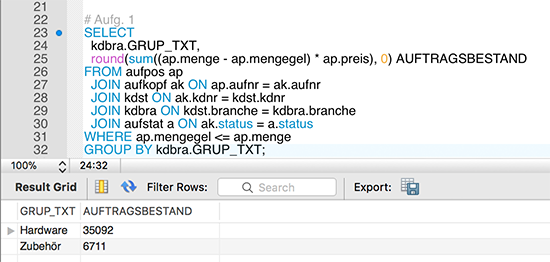
\includegraphics{mat_inf1}

\subsection{}
Lassen Sie sich bitte die (Lager-)bestände derjenigen Artikel anzeigen, von denen keine Aufträge vorliegen. Die Ergebnistabelle soll nach dem Bestand sortiert vorliegen und folgendermaßen aussehen:

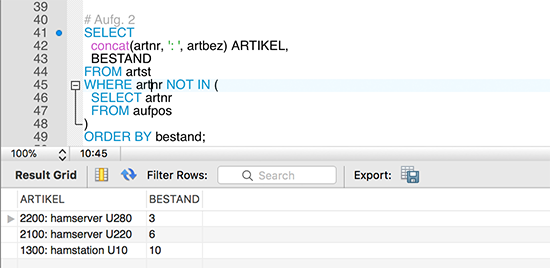
\includegraphics{mat_inf2}

\subsection{}
Lassen Sie sich bitte die wertmäßigen Abweichungen der Auftragsbestände zwischen dem normalen Verkaufspreis im Artikelstamm und dem für den jeweiligen Auftrag gültigen Preis (in Auftragsposition) für alle Auftragspositionen mit einer derartigen Abweichung anzeigen. Die Ergebnistabelle soll folgendermaßen aussehen:

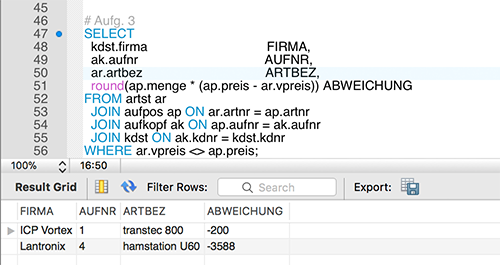
\includegraphics{mat_inf3}

\subsection{}
Es sollen alle Kunden angezeigt werden und von denjenigen Kunden, die etwas bestellt haben, soll deren Auftragsnummer für den jeweiligen Auftrag ebenfalls angezeigt werden. Um die Ergebnistabelle lesbarer zu machen, soll für diejenigen Kunden, die nichts bestellt haben, die (fehlende) Auftragsnummer nicht als Nullwert angezeigt werden, sondern als Ziffer 0. Ebenfalls sollen die Adressdaten innerhalb einer Spalte entsprechend formatiert ausgegeben werden (vgl. Beispieltabelle). Eine Sortierung nach der Kundennummer soll erfolgen.

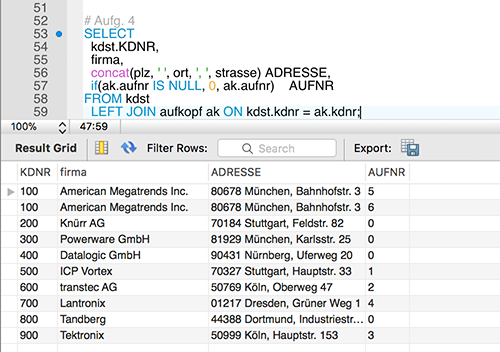
\includegraphics{mat_inf4}

\pagebreak
\setcounter{subsection}{0}
\section* {Aufgaben company:}

\subsection{}
Suchen Sie bitte die Nummern und Städte der Lieferanten, die in derselben Stadt wie Lieferant \glqq S1\grqq\ und \glqq S2\grqq\ ihren Firmensitz haben. Die Ergebnistabelle soll folgendermaßen aussehen:

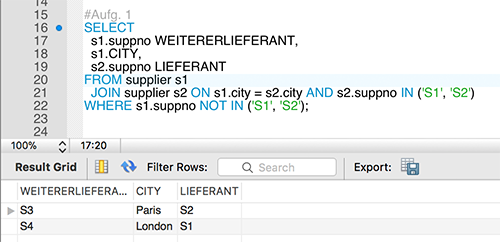
\includegraphics{company1}

\subsection{}
Lassen Sie bitte alle Angestellten auflisten, die denselben Job wie „FORD“ haben. Schließen Sie hierbei die Anzeige von „FORD“ selbst aus.

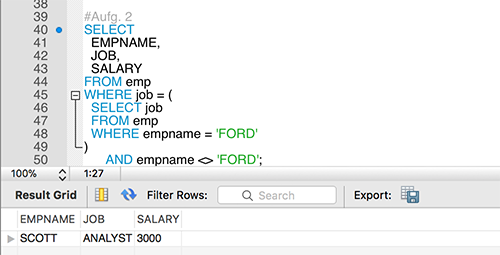
\includegraphics{company2}

\subsection{}
Lassen Sie sich bitte alle Angestellten mit Lohn, Job, Name und Abteilungsnummer nach dem Lohn absteigend sortiert auflisten, die mehr verdienen als der am besten bezahlte Angestellte in Abteilung 30.

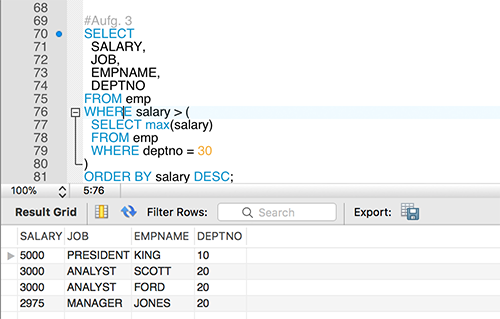
\includegraphics{company3}

\pagebreak
\subsection{}
Lassen Sie sich bitte alle Angestellten in Abteilung 10 auflisten, die einen Job haben, wie ihn auch irgendein Angestellter in Abteilung 30 hat.

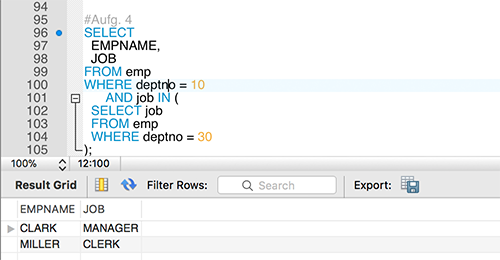
\includegraphics{company4}

\subsection{}
Entwickeln Sie bitte eine eigene Aufgabenstellung und die entsprechende Lösung. Dokumentieren Sie die Aufgabenstellung! Die Übungsdatenbank kann mat\_inf oder company sein. Bedingung: es sollen mindestens eine Unteranfrage und ein Join enthalten sein.
\\\\
\textbf {Aufgabe:} Lassen Sie sich bitte die Wertmäßige Abweichung des Gehalts vom Durchschnittsgehalt der jeweiligen Abteilung von denjenigen Mitarbeitern auflisten, die vor 2010 eingestellt wurden. In der Tabelle soll weiterhin das Durchschnittsgehalt und der Name der Abteilung und die Nummer, der Name, das Anstellungsdatum und das Gehalt des Mitarbeiters  angezeigt werden. Die Tabelle soll nach Abteilungsname und Höhe der Abweichung sortiert sein.

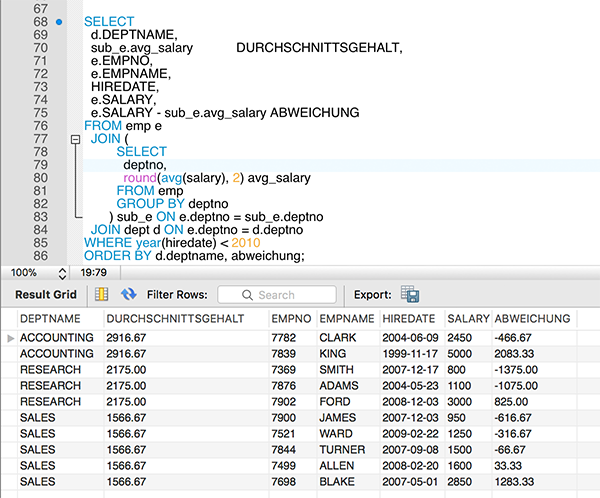
\includegraphics{companyEig}


\end{document}
